\documentclass[tikz,border=8pt]{standalone}
\usepackage[T1]{fontenc}
\usepackage[scaled=0.88]{helvet}
\usepackage{amsmath,amssymb}
\usepackage{tikz}
\usetikzlibrary{arrows.meta,positioning,shapes.geometric,shapes.misc,calc,fit,backgrounds}

\begin{document}
\sffamily
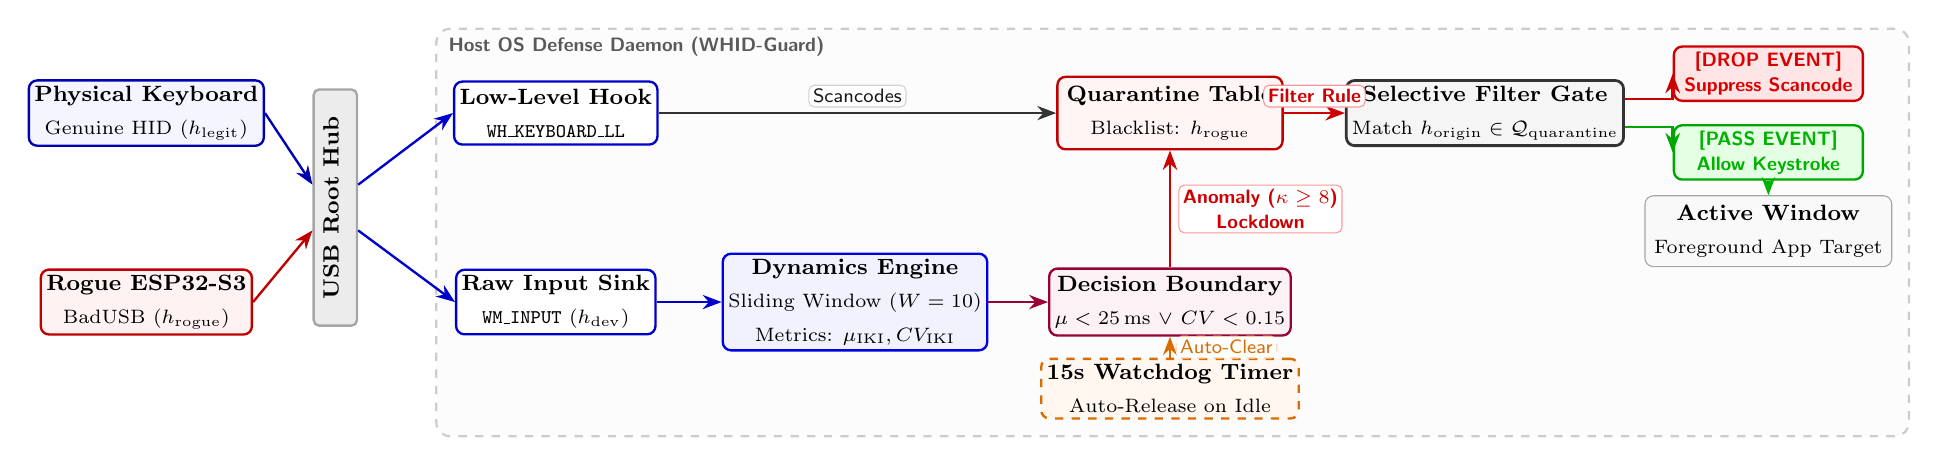
\begin{tikzpicture}[
    >=Stealth,
    font=\small,
    % Device blocks
    dev_rogue/.style={
        rectangle,
        rounded corners=3pt,
        draw=red!75!black,
        line width=0.85pt,
        fill=red!5!white,
        minimum width=2.4cm,
        minimum height=0.80cm,
        inner sep=2pt,
        align=center
    },
    dev_legit/.style={
        rectangle,
        rounded corners=3pt,
        draw=blue!70!black,
        line width=0.85pt,
        fill=blue!4!white,
        minimum width=2.4cm,
        minimum height=0.80cm,
        inner sep=2pt,
        align=center
    },
    % Module block
    mod_block/.style={
        rectangle,
        rounded corners=3pt,
        draw=blue!80!black,
        line width=0.85pt,
        fill=white,
        minimum width=2.4cm,
        minimum height=0.80cm,
        inner sep=2pt,
        align=center
    },
    % Engine block
    eng_block/.style={
        rectangle,
        rounded corners=3pt,
        draw=blue!90!black,
        line width=0.85pt,
        fill=blue!5!white,
        minimum width=2.5cm,
        minimum height=0.85cm,
        inner sep=2pt,
        align=center
    },
    % Decision Box
    decision_box/.style={
        rectangle,
        rounded corners=3pt,
        draw=purple!80!black,
        line width=0.85pt,
        fill=purple!5!white,
        minimum width=2.5cm,
        minimum height=0.85cm,
        inner sep=2pt,
        align=center
    },
    % Gate switch
    gate_block/.style={
        rectangle,
        rounded corners=3pt,
        draw=black!80,
        line width=1.0pt,
        fill=gray!8!white,
        minimum width=2.5cm,
        minimum height=0.80cm,
        inner sep=2pt,
        align=center
    },
    % Action pills
    pill_drop/.style={
        rectangle,
        rounded corners=3pt,
        draw=red!80!black,
        line width=0.85pt,
        fill=red!10!white,
        minimum width=2.4cm,
        minimum height=0.60cm,
        inner sep=2pt,
        align=center,
        font=\sffamily\scriptsize\bfseries,
        text=red!85!black
    },
    pill_pass/.style={
        rectangle,
        rounded corners=3pt,
        draw=green!65!black,
        line width=0.85pt,
        fill=green!10!white,
        minimum width=2.4cm,
        minimum height=0.60cm,
        inner sep=2pt,
        align=center,
        font=\sffamily\scriptsize\bfseries,
        text=green!70!black
    },
    % Watchdog
    wdt_block/.style={
        rectangle,
        rounded corners=3pt,
        draw=orange!85!black,
        line width=0.85pt,
        dashed,
        fill=orange!6!white,
        minimum width=2.5cm,
        minimum height=0.60cm,
        inner sep=2pt,
        align=center
    },
    % Badges
    badge/.style={
        font=\sffamily\scriptsize,
        fill=white,
        draw=gray!35,
        line width=0.4pt,
        rounded corners=2pt,
        inner sep=1.5pt,
        align=center,
        text=black!90
    },
    badge_red/.style={
        font=\sffamily\scriptsize\bfseries,
        fill=white,
        draw=red!40,
        line width=0.4pt,
        rounded corners=2pt,
        inner sep=1.5pt,
        align=center,
        text=red!80!black
    },
    badge_green/.style={
        font=\sffamily\scriptsize\bfseries,
        fill=white,
        draw=green!40,
        line width=0.4pt,
        rounded corners=2pt,
        inner sep=1.5pt,
        align=center,
        text=green!70!black
    },
    badge_amber/.style={
        font=\sffamily\scriptsize,
        fill=white,
        draw=orange!40,
        line width=0.4pt,
        rounded corners=2pt,
        inner sep=1.5pt,
        align=center,
        text=orange!85!black
    }
]

% ==============================================================================
% Column 1: Physical Peripherals (x = 1.2)
% ==============================================================================
\node[dev_legit] (kb_legit) at (1.2, 1.2) {
    \textbf{\footnotesize Physical Keyboard}\\[1pt]
    \scriptsize Genuine HID ($h_{\text{legit}}$)
};

\node[dev_rogue] (badusb) at (1.2, -1.2) {
    \textbf{\footnotesize Rogue ESP32-S3}\\[1pt]
    \scriptsize BadUSB ($h_{\text{rogue}}$)
};

% Column 2: Host USB Bus (x = 3.6)
\node[rectangle, draw=gray!70, fill=gray!15, line width=0.85pt, minimum width=0.55cm, minimum height=3.0cm, rounded corners=2pt, align=center] (bus) at (3.6, 0.0) {
    \rotatebox{90}{\textbf{\footnotesize USB Root Hub}}
};

\draw[->, line width=0.85pt, draw=blue!70!black] (kb_legit.east) -- (bus.135);
\draw[->, line width=0.85pt, draw=red!75!black]  (badusb.east)   -- (bus.225);

% ==============================================================================
% Column 3: Parallel Ingestion Channels (x = 6.4)
% ==============================================================================
\node[mod_block] (hook) at (6.4, 1.2) {
    \textbf{\footnotesize Low-Level Hook}\\[1pt]
    \scriptsize \texttt{WH\_KEYBOARD\_LL}
};

\node[mod_block] (rawinput) at (6.4, -1.2) {
    \textbf{\footnotesize Raw Input Sink}\\[1pt]
    \scriptsize \texttt{WM\_INPUT} ($h_{\text{dev}}$)
};

\draw[->, line width=0.85pt, draw=blue!80!black] (bus.45) -- (hook.west);
\draw[->, line width=0.85pt, draw=blue!80!black] (bus.315) -- (rawinput.west);

% ==============================================================================
% Column 4: Dynamics Engine (x = 10.2)
% ==============================================================================
\node[eng_block] (engine) at (10.2, -1.2) {
    \textbf{\footnotesize Dynamics Engine}\\[1pt]
    \scriptsize Sliding Window ($W=10$)\\[1pt]
    \scriptsize Metrics: $\mu_{\text{IKI}}, CV_{\text{IKI}}$
};
\draw[->, line width=0.85pt, draw=blue!80!black] (rawinput.east) -- (engine.west);

% ==============================================================================
% Column 5: Decision Boundary & Quarantine Blacklist (x = 14.2)
% ==============================================================================
\node[rectangle, rounded corners=3pt, draw=red!75!black, line width=0.85pt, fill=red!4!white, minimum width=2.6cm, minimum height=0.80cm, align=center] (qset) at (14.2, 1.2) {
    \textbf{\footnotesize Quarantine Table}\\[1pt]
    \scriptsize Blacklist: $h_{\text{rogue}}$
};

\node[decision_box] (decision_box) at (14.2, -1.2) {
    \textbf{\footnotesize Decision Boundary}\\[1pt]
    \scriptsize $\mu < 25$\,ms $\lor$ $CV < 0.15$
};
\draw[->, line width=0.85pt, draw=purple!80!black] (engine.east) -- (decision_box.west);

% Vertical Quarantine update from Decision Box to Q-Set
\draw[->, line width=0.9pt, draw=red!80!black] (decision_box.north) -- node[right=3pt, badge_red] {Anomaly ($\kappa \ge 8$)\\[1pt]Lockdown} (qset.south);

% Watchdog Timer (Below Decision Box)
\node[wdt_block] (wdt) at (14.2, -2.3) {
    \textbf{\footnotesize 15s Watchdog Timer}\\[1pt]
    \scriptsize Auto-Release on Idle
};
\draw[->, line width=0.8pt, dashed, draw=orange!85!black] (wdt.north) -- node[right=2pt, badge_amber] {Auto-Clear} (decision_box.south);

% ==============================================================================
% Column 6: Selective Filter Gate (x = 18.2)
% ==============================================================================
\node[gate_block] (gate) at (18.2, 1.2) {
    \textbf{\footnotesize Selective Filter Gate}\\[1pt]
    \scriptsize Match $h_{\text{origin}} \in \mathcal{Q}_{\text{quarantine}}$
};

% Scancodes and Blacklist filter into Gate
\draw[->, line width=0.85pt, draw=black!80] (hook.east) -- node[above=2pt, badge] {Scancodes} (qset.west);
\draw[->, line width=0.9pt, draw=red!80!black] (qset.east) -- node[above=2pt, badge_red] {Filter Rule} (gate.west);

% ==============================================================================
% Column 7: Enforcement Outputs (x = 21.8)
% ==============================================================================
\node[pill_drop] (drop_out) at (21.8, 1.7) {\textbf{[DROP EVENT]}\\[1pt]\scriptsize Suppress Scancode};
\node[pill_pass] (pass_out) at (21.8, 0.7) {\textbf{[PASS EVENT]}\\[1pt]\scriptsize Allow Keystroke};

% Routing from Gate to Outputs (Clean straight orthogonal lines)
\draw[->, line width=0.9pt, draw=red!80!black] ([yshift=5pt]gate.east) -| (drop_out.west);
\draw[->, line width=0.9pt, draw=green!65!black] ([yshift=-5pt]gate.east) -| (pass_out.west);

% Active Application Window
\node[rectangle, rounded corners=3pt, draw=gray!70, fill=gray!5, minimum width=2.4cm, minimum height=0.60cm, align=center] (target_app) at (21.8, -0.3) {
    \textbf{\footnotesize Active Window}\\[1pt]
    \scriptsize Foreground App Target
};

\draw[->, line width=0.8pt, draw=green!70!black] (pass_out.south) -- (target_app.north);

% Background Container
\begin{scope}[on background layer]
    \node[rectangle, draw=gray!40, dashed, fill=gray!2, line width=0.8pt, rounded corners=5pt,
          fit=(hook) (rawinput) (engine) (decision_box) (qset) (wdt) (gate) (drop_out) (pass_out) (target_app),
          inner sep=6pt] (host_bg) {};
    \node[anchor=north west, font=\sffamily\bfseries\scriptsize, text=gray!70!black] at (host_bg.north west) {\,Host OS Defense Daemon (WHID-Guard)};
\end{scope}

\end{tikzpicture}
\end{document}
